% !TEX root = ../Report.tex
\section{Data Analysis}
\label{sec:data_analysis}

\begin{figure*}[t]
    \centering
    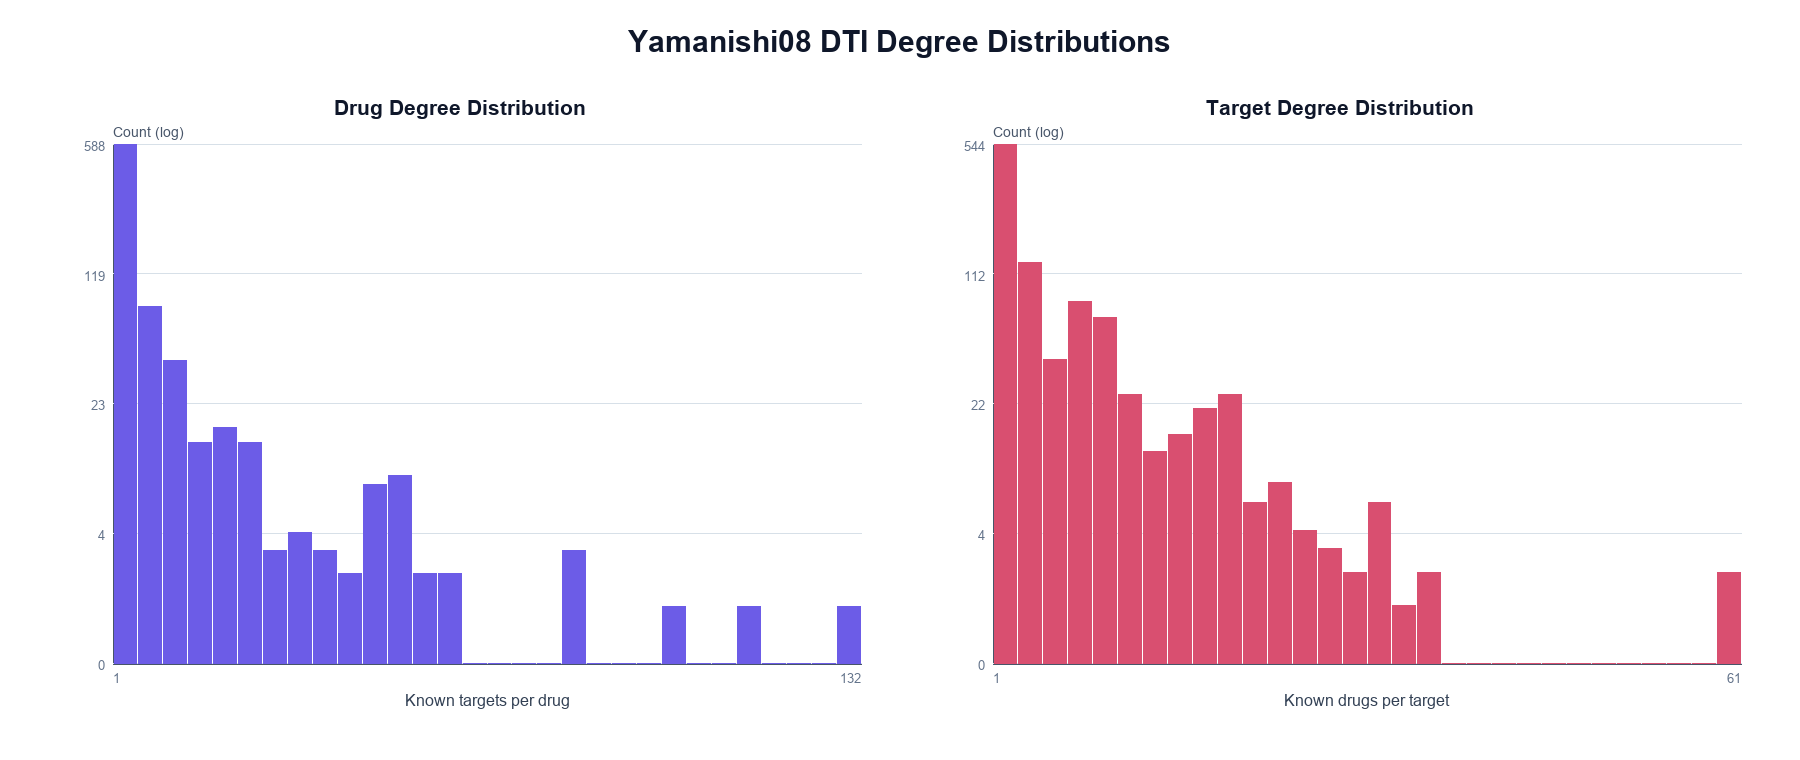
\includegraphics[width=0.9\textwidth]{images/data_analysis/dti_degree_distribution.png}
    \caption{Degree distributions of drugs and targets in the Yamanishi08 DTI network. The log-scale counts show that most entities have few known interactions, while a small number of drugs and targets act as high-degree hubs.}
    \Description{Two log-scale histograms showing known targets per drug and known drugs per target in the Yamanishi08 DTI network, with many low-degree entities and a few high-degree hubs.}
    \label{fig:dti_degree_distribution}
\end{figure*}
The experiments use the Yamanishi08 benchmark for drug--target interaction prediction. The DTI network contains 5,127 known positive interactions between 791 drugs and 989 target proteins. These positives occupy only 0.6554\% of the 782,299 possible drug--target pairs, so the task is sparse at the interaction level. Unobserved pairs are sampled as negatives for training and evaluation, but they are not experimentally confirmed non-interactions.

\begin{table}[t]
\centering
\caption{Key statistics of the Yamanishi08 DTI data and auxiliary knowledge graph.}
\label{tab:dataset_stats}
\small
\begin{tabular}{lr}
\toprule
\textbf{Statistic} & \textbf{Value} \\
\midrule
Known positive interactions & 5,127 \\
Unique drugs & 791 \\
Unique target proteins & 989 \\
Possible drug--target pairs & 782,299 \\
Observed positive density & 0.6554\% \\
Average targets per drug & 6.48 \\
Average drugs per target & 5.18 \\
Auxiliary KG triples & 95,579 \\
Auxiliary KG entities & 25,487 \\
Auxiliary KG relation types & 48 \\
\bottomrule
\end{tabular}
\end{table}

Each drug is represented by a 1,024-dimensional Morgan fingerprint and each protein by a 147-dimensional CTD descriptor. The auxiliary knowledge graph covers all evaluated drugs and targets, providing 95,579 unique biomedical triples over 25,487 entities and 48 relation types. The warm-start protocol evaluates unseen drug--target pairs while keeping test drugs and proteins present in training.


Figure~\ref{fig:dti_degree_distribution} shows that the interaction evidence is also long-tailed at the entity level. Most drugs and targets have only a few known interactions, while a small number of hubs have many. In the underlying statistics, 74.3\% of drugs have at most five known targets and 55.0\% of targets have at most two known drugs.

This structure motivates models that do not rely only on direct DTI frequency. KG embeddings can provide graph-derived context for low-degree drugs and targets, and CompGCN-style message passing can propagate information through typed biomedical relations before the downstream NFM combines graph, molecular, and sequence features.
